\section{Topic}
	\subsection{Brief Task Description}
	This project is about implementing the game Pong on the Atlys Spartan-6 FPGA board. Pong is a two dimensional multiplayer game that simulates table-tennis. Each of the two players controls an in game paddle by moving it vertically in order to hit a ball back and forth. A player scores a point when the opponent fails to return the ball. 
	
	We also took advantage of the built-in HDMI port and the AC-97 Codec to produce a better image and audio quality output. 
	
	Figure \ref{board+screenshot} shows a picture of the used board, and a screenshot of the (yet to be) realized game. 
	
	\begin{figure}[h]
		\begin{subfigure}[b]{.4\textwidth}
			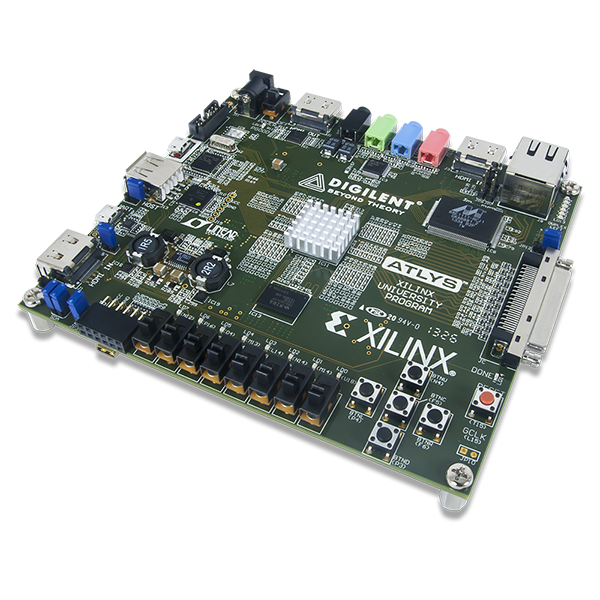
\includegraphics[width=8cm]{images/atlys_pic.png}
			\caption{Atlys Spartan-6 board}
		\end{subfigure}
		\hfill
		\begin{subfigure}[b]{.4\textwidth}
			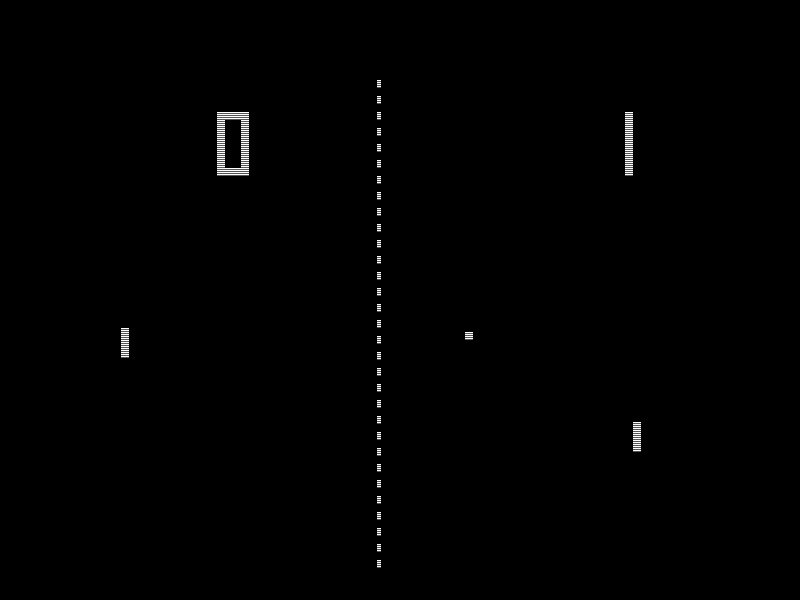
\includegraphics[width=8cm]{images/pong_screenshot.png}		
			\caption{Screenshot of the game Pong}
		\end{subfigure}
		
	\caption{Used board and screenshot of the game}
	\label{board+screenshot}
	\end{figure}
	
	
	\subsection{Block Diagram}
	\subsection{Functional Details}
